% Options for packages loaded elsewhere
\PassOptionsToPackage{unicode}{hyperref}
\PassOptionsToPackage{hyphens}{url}
\PassOptionsToPackage{dvipsnames,svgnames,x11names}{xcolor}
%
\documentclass[
  letterpaper,
  DIV=11,
  numbers=noendperiod]{scrartcl}

\usepackage{amsmath,amssymb}
\usepackage{iftex}
\ifPDFTeX
  \usepackage[T1]{fontenc}
  \usepackage[utf8]{inputenc}
  \usepackage{textcomp} % provide euro and other symbols
\else % if luatex or xetex
  \usepackage{unicode-math}
  \defaultfontfeatures{Scale=MatchLowercase}
  \defaultfontfeatures[\rmfamily]{Ligatures=TeX,Scale=1}
\fi
\usepackage{lmodern}
\ifPDFTeX\else  
    % xetex/luatex font selection
\fi
% Use upquote if available, for straight quotes in verbatim environments
\IfFileExists{upquote.sty}{\usepackage{upquote}}{}
\IfFileExists{microtype.sty}{% use microtype if available
  \usepackage[]{microtype}
  \UseMicrotypeSet[protrusion]{basicmath} % disable protrusion for tt fonts
}{}
\makeatletter
\@ifundefined{KOMAClassName}{% if non-KOMA class
  \IfFileExists{parskip.sty}{%
    \usepackage{parskip}
  }{% else
    \setlength{\parindent}{0pt}
    \setlength{\parskip}{6pt plus 2pt minus 1pt}}
}{% if KOMA class
  \KOMAoptions{parskip=half}}
\makeatother
\usepackage{xcolor}
\setlength{\emergencystretch}{3em} % prevent overfull lines
\setcounter{secnumdepth}{-\maxdimen} % remove section numbering
% Make \paragraph and \subparagraph free-standing
\ifx\paragraph\undefined\else
  \let\oldparagraph\paragraph
  \renewcommand{\paragraph}[1]{\oldparagraph{#1}\mbox{}}
\fi
\ifx\subparagraph\undefined\else
  \let\oldsubparagraph\subparagraph
  \renewcommand{\subparagraph}[1]{\oldsubparagraph{#1}\mbox{}}
\fi


\providecommand{\tightlist}{%
  \setlength{\itemsep}{0pt}\setlength{\parskip}{0pt}}\usepackage{longtable,booktabs,array}
\usepackage{calc} % for calculating minipage widths
% Correct order of tables after \paragraph or \subparagraph
\usepackage{etoolbox}
\makeatletter
\patchcmd\longtable{\par}{\if@noskipsec\mbox{}\fi\par}{}{}
\makeatother
% Allow footnotes in longtable head/foot
\IfFileExists{footnotehyper.sty}{\usepackage{footnotehyper}}{\usepackage{footnote}}
\makesavenoteenv{longtable}
\usepackage{graphicx}
\makeatletter
\def\maxwidth{\ifdim\Gin@nat@width>\linewidth\linewidth\else\Gin@nat@width\fi}
\def\maxheight{\ifdim\Gin@nat@height>\textheight\textheight\else\Gin@nat@height\fi}
\makeatother
% Scale images if necessary, so that they will not overflow the page
% margins by default, and it is still possible to overwrite the defaults
% using explicit options in \includegraphics[width, height, ...]{}
\setkeys{Gin}{width=\maxwidth,height=\maxheight,keepaspectratio}
% Set default figure placement to htbp
\makeatletter
\def\fps@figure{htbp}
\makeatother

\KOMAoption{captions}{tableheading}
\makeatletter
\@ifpackageloaded{caption}{}{\usepackage{caption}}
\AtBeginDocument{%
\ifdefined\contentsname
  \renewcommand*\contentsname{Table of contents}
\else
  \newcommand\contentsname{Table of contents}
\fi
\ifdefined\listfigurename
  \renewcommand*\listfigurename{List of Figures}
\else
  \newcommand\listfigurename{List of Figures}
\fi
\ifdefined\listtablename
  \renewcommand*\listtablename{List of Tables}
\else
  \newcommand\listtablename{List of Tables}
\fi
\ifdefined\figurename
  \renewcommand*\figurename{Figure}
\else
  \newcommand\figurename{Figure}
\fi
\ifdefined\tablename
  \renewcommand*\tablename{Table}
\else
  \newcommand\tablename{Table}
\fi
}
\@ifpackageloaded{float}{}{\usepackage{float}}
\floatstyle{ruled}
\@ifundefined{c@chapter}{\newfloat{codelisting}{h}{lop}}{\newfloat{codelisting}{h}{lop}[chapter]}
\floatname{codelisting}{Listing}
\newcommand*\listoflistings{\listof{codelisting}{List of Listings}}
\makeatother
\makeatletter
\makeatother
\makeatletter
\@ifpackageloaded{caption}{}{\usepackage{caption}}
\@ifpackageloaded{subcaption}{}{\usepackage{subcaption}}
\makeatother
\ifLuaTeX
  \usepackage{selnolig}  % disable illegal ligatures
\fi
\usepackage{bookmark}

\IfFileExists{xurl.sty}{\usepackage{xurl}}{} % add URL line breaks if available
\urlstyle{same} % disable monospaced font for URLs
\hypersetup{
  pdftitle={Week 8 - Introduction to Regression and Correlation Models},
  colorlinks=true,
  linkcolor={blue},
  filecolor={Maroon},
  citecolor={Blue},
  urlcolor={Blue},
  pdfcreator={LaTeX via pandoc}}

\title{Week 8 - Introduction to Regression and Correlation Models}
\author{}
\date{}

\begin{document}
\maketitle

\subsection{Introduction:}\label{introduction}

Welcome to this seminar on linear regression in the context of
mathematical modeling. Linear regression and Correlation are related
statistical techniques used to model the relationship between one or
more independent variables and a dependent variable.

In this seminar, we will explore the principles of linear regression,
correlation, and confidence intervals. We will also look at its
applications, and how it fits into mathematical modeling.

\subsection{Understanding
Correlations}\label{understanding-correlations}

We may be interested in seeing if there is a linear relationship between
2 (scale) variables.

We can plot the values on a scatter diagram and see how close the points
are to a straight line

Consider the following plot, where each point is one data point. Each
point represents the data for one person. The scatterplot displays two
numerical variables, x (independent or predictor) and y (dependent)

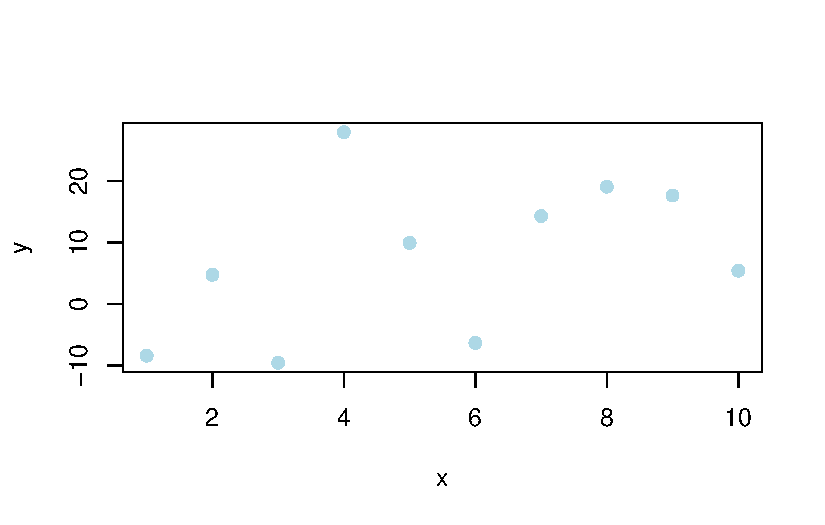
\includegraphics{Week8a_files/figure-pdf/unnamed-chunk-1-1.pdf}

The relationship between the two variables is not exact -- there is an
unpredictable or random element: every person is different.

We can model the underlying relationship by a straight line of best fit
(or trendline) We can measure how close those points are to that line
(below, the trendline is in red)

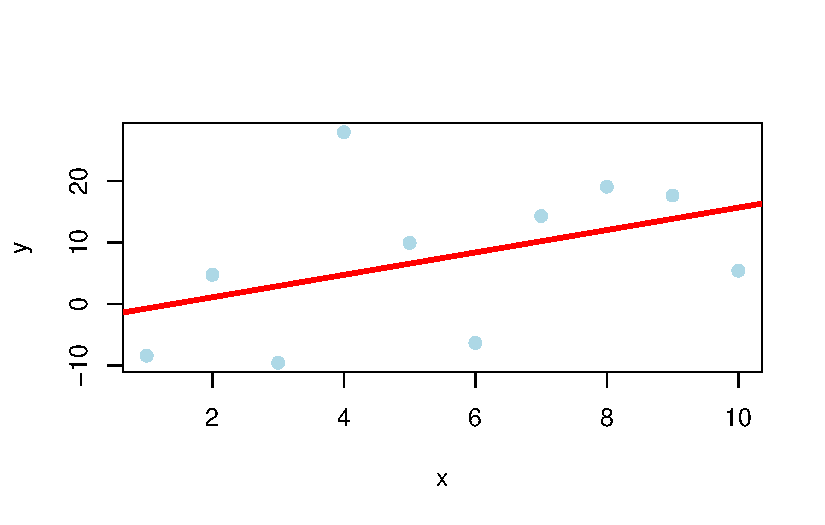
\includegraphics{Week8a_files/figure-pdf/unnamed-chunk-2-1.pdf}

\subsection{Pearsons Product Moment Correlation,
r}\label{pearsons-product-moment-correlation-r}

The correlation coefficient, r, measures how close the points are to the
line ie. the strength of the linear relationship.

\[ r = \frac{S_{xy}}{\sqrt{S_{xx}S_{yy}}} \] where:

\[ S_{xy} = \sum(x - \bar{x})(y - \bar{y}) = \sum xy - \frac{\sum x \sum y}{n})  \]

\[ s_{xx} = \sum(x - \bar{x})^2 = \sum x^2 - \frac{(\sum x)^2}{n} \]
\[ s_{yy} = \sum(y - \bar{y})^2 = \sum y^2 - \frac{(\sum y)^2}{n} \] -
Its value is between -1 and 1 - A value close to 1 or -1 represents a
strong linear relationship. -A positive value suggests a positive
relationship ie. as one variable increases the other increases - A
negative value suggests a negative relationship ie. as one variable
increases the other decreases - A value close to 0 means a very weak or
no linear relationship.

(Note that even if there is no linear relationship, there still may be a
relationship which is non-linear)

\section{Plots with strong positive, strong negative, no correlation,
perfect negative
correlation}\label{plots-with-strong-positive-strong-negative-no-correlation-perfect-negative-correlation}

Consider the following example. The number of vehicles, 𝑥 millions, and
the number of accidents, 𝑦 thousands, in 15 different countries were:

\begin{longtable}[]{@{}
  >{\raggedright\arraybackslash}p{(\columnwidth - 30\tabcolsep) * \real{0.1667}}
  >{\raggedright\arraybackslash}p{(\columnwidth - 30\tabcolsep) * \real{0.0556}}
  >{\raggedright\arraybackslash}p{(\columnwidth - 30\tabcolsep) * \real{0.0556}}
  >{\raggedright\arraybackslash}p{(\columnwidth - 30\tabcolsep) * \real{0.0556}}
  >{\raggedright\arraybackslash}p{(\columnwidth - 30\tabcolsep) * \real{0.0556}}
  >{\raggedright\arraybackslash}p{(\columnwidth - 30\tabcolsep) * \real{0.0556}}
  >{\raggedright\arraybackslash}p{(\columnwidth - 30\tabcolsep) * \real{0.0556}}
  >{\raggedright\arraybackslash}p{(\columnwidth - 30\tabcolsep) * \real{0.0556}}
  >{\raggedright\arraybackslash}p{(\columnwidth - 30\tabcolsep) * \real{0.0556}}
  >{\raggedright\arraybackslash}p{(\columnwidth - 30\tabcolsep) * \real{0.0556}}
  >{\raggedright\arraybackslash}p{(\columnwidth - 30\tabcolsep) * \real{0.0556}}
  >{\raggedright\arraybackslash}p{(\columnwidth - 30\tabcolsep) * \real{0.0556}}
  >{\raggedright\arraybackslash}p{(\columnwidth - 30\tabcolsep) * \real{0.0556}}
  >{\raggedright\arraybackslash}p{(\columnwidth - 30\tabcolsep) * \real{0.0556}}
  >{\raggedright\arraybackslash}p{(\columnwidth - 30\tabcolsep) * \real{0.0556}}
  >{\raggedright\arraybackslash}p{(\columnwidth - 30\tabcolsep) * \real{0.0556}}@{}}
\toprule\noalign{}
\begin{minipage}[b]{\linewidth}\raggedright
Country
\end{minipage} & \begin{minipage}[b]{\linewidth}\raggedright
A
\end{minipage} & \begin{minipage}[b]{\linewidth}\raggedright
B
\end{minipage} & \begin{minipage}[b]{\linewidth}\raggedright
C
\end{minipage} & \begin{minipage}[b]{\linewidth}\raggedright
D
\end{minipage} & \begin{minipage}[b]{\linewidth}\raggedright
E
\end{minipage} & \begin{minipage}[b]{\linewidth}\raggedright
F
\end{minipage} & \begin{minipage}[b]{\linewidth}\raggedright
G
\end{minipage} & \begin{minipage}[b]{\linewidth}\raggedright
H
\end{minipage} & \begin{minipage}[b]{\linewidth}\raggedright
I
\end{minipage} & \begin{minipage}[b]{\linewidth}\raggedright
J
\end{minipage} & \begin{minipage}[b]{\linewidth}\raggedright
K
\end{minipage} & \begin{minipage}[b]{\linewidth}\raggedright
L
\end{minipage} & \begin{minipage}[b]{\linewidth}\raggedright
M
\end{minipage} & \begin{minipage}[b]{\linewidth}\raggedright
N
\end{minipage} & \begin{minipage}[b]{\linewidth}\raggedright
O
\end{minipage} \\
\midrule\noalign{}
\endhead
\bottomrule\noalign{}
\endlastfoot
Vehicles (x) millions & 8.6 & 13.4 & 12.8 & 9.3 & 1.3 & 9.4 & 13.1 & 4.9
& 13.5 & 9.6 & 7.5 & 9.8 & 23.3 & 21 & 19.4 \\
Accidents (y) thousands & 33 & 51 & 30 & 48 & 12 & 23 & 46 & 18 & 36 &
50 & 34 & 35 & 95 & 99 & 69 \\
\end{longtable}

Calculate the product moment correlation coefficient for the number of
vehicle and the number of accidents.

We will need the following

\[ \sum x = 176.9  \sum y = 679 \]
\[ \sum x^2 = 2576.47  \sum y^2 = 39771 \] \[ \sum xy = 9915.3 \]

\[ S_{xy}  = \sum xy - \frac{\sum x \sum y}{n} = 9915.3 - \frac{176.9 * 679}{15} = 1907.62... \]

\[ s_{xx} = \sum x^2 - \frac{(\sum x)^2}{n} = 257.47 - \frac{(176.9)^2}{15} = 490.22... \]
\[ s_{yy} = \sum y^2 - \frac{(\sum y)^2}{n} = 39771 - \frac{(679)^2}{15} = 9034.93... \]
\[ r = \frac{S_{xy}}{\sqrt{S_{xx}S_{yy}}} = \frac{1907.62...}{\sqrt{490.22...*9034.93...}} = 0.906(3.d.p)\]

This suggests a very strong positive linear relationship between the
number of vehicles and the number of accidents.

Consider the following example. The head circumference in cm (x) and
gestation period (y) in weeks for new born babies at a certain clinic
over a period of time is as follows.

\begin{longtable}[]{@{}lllllll@{}}
\toprule\noalign{}
Baby & A & B & C & D & E & F \\
\midrule\noalign{}
\endhead
\bottomrule\noalign{}
\endlastfoot
Head circumference (x) & 31.1 & 33.3 & 30.0 & 31.5 & 35.0 & 30.2 \\
Gestation period (y) & 36 & 37 & 38 & 38 & 40 & 40 \\
\end{longtable}

Find the correlation between head circumference and gestation period.

We will need the following

\[ \sum x = 191.1  \sum y = 229 \]
\[ \sum x^2 = 6105.39  \sum y^2 = 8753 \] \[ \sum xy = 7296.7 \]

\[ S_{xy}  = \sum xy - \frac{\sum x \sum y}{n} = 7296.7 - \frac{191.1 * 229}{6} = 3.05 \]

\[ s_{xx} = \sum x^2 - \frac{(\sum x)^2}{n} = 6105.39 - \frac{(191.1)^2}{6} = 18.855 \]
\[ s_{yy} = \sum y^2 - \frac{(\sum y)^2}{n} = 8753 - \frac{(229)^2}{6} = 12.833 \]
\[ r = \frac{S_{xy}}{\sqrt{S_{xx}S_{yy}}} = \frac{3.05}{\sqrt{18.855*12.833}} = 0.196\]
This is a low correlation which suggests very little evidence of a
linear relationship between head circumference and gestation period

\subsection{Some problems}\label{some-problems}

A very strong correlation does not necessarily mean that a change in x
causes a change in y

A very weak correlation does not necessarily mean that x and y are
unrelated. The relationship could be non-linear.

High correlations can arise purely by chance, particularly if the sample
size is small. The correlation may not be significantly different from
zero.

\subsection{Understanding Linear
Regression:}\label{understanding-linear-regression}

Linear regression aims to establish a linear relationship between
independent variables (predictors) and a dependent variable (response).
It assumes that this relationship can be expressed as a linear equation:
Y = β₀ + β₁X₁ + β₂X₂ + \ldots{} + βₖXₖ + ε, where: Y is the dependent
variable. X₁, X₂, \ldots, Xₖ are the independent variables. β₀, β₁, β₂,
\ldots, βₖ are the coefficients. ε represents the error term, accounting
for unexplained variability.

\subsection{Simple Linear Regression:}\label{simple-linear-regression}

In simple linear regression, there is only one independent variable (X)
and one dependent variable (Y). The relationship is expressed as
\(y=a+bx\). The goal is to find the best-fitting line that minimizes the
sum of squared errors (residuals) between the predicted and actual
values of Y.

a is the intercept of the line.\\
b is the slope of the line.

In order to calculate a and b, you need the following

\[ a = \bar{y} - b\bar{x}\] and

\[ b = \frac{S_{xy}}{S_{xx}} \] Wait, we've seen the terms \$
S\_\{xy\}\$ and \(S_{xx}\) before when working out correlation!

Example: The results from an experiment in which different masses were
placed on a spring and the resulting length of the spring measured, are
shown below

\begin{longtable}[]{@{}llllll@{}}
\toprule\noalign{}
Mass, x (kg) & 20 & 40 & 60 & 80 & 100 \\
\midrule\noalign{}
\endhead
\bottomrule\noalign{}
\endlastfoot
Length, y (cm) & 48 & 55.1 & 56.3 & 61.2 & 68 \\
\end{longtable}

We will need the following

\[ \sum x = 300, \sum y = 288.6 \] \[ \sum x^2 = 22000 \]
\[ \bar x = 60, \bar y = 57.72 \] \[ \sum xy = 18238 \]

\[ S_{xy}  = \sum xy - \frac{\sum x \sum y}{n} = 18238 - \frac{300 * 288.6}{5} = 922 \]

\[ s_{xx} = \sum x^2 - \frac{(\sum x)^2}{n} = 22000 - \frac{(300)^2}{5} = 4000 \]
\[ b = \frac{S_{xy}}{S_{xx}} = \frac{922}{4000}\]
\[ a = \bar y - b\bar x = 57.72 - 0.2305 * 60 = 43.89\]
\[ y = 43.89 + 0.2305x \] Predict and interpret:

\begin{enumerate}
\def\labelenumi{\alph{enumi}.}
\tightlist
\item
  the value of y when the mass x = 35 kg
\item
  the value of y when the mass x = 120 kg
\end{enumerate}

\begin{enumerate}
\def\labelenumi{\alph{enumi})}
\item
  \[y=43.89+0.2305*35=52.0 cm \] If the mass is 35 kg, then the length
  of the spring will be 52 cm on average
\item
  \[y=43.89+0.2305*120=71.55 cm \] If the mass is 120 kg, then the
  length of the spring will be 71.6 cm on average
\end{enumerate}

In terms of predicting new values for the above example. The range of
observed values of x was from 20 to 100. If we predict the value of Y
for 20≤𝑥≤100, this is called INTERPOLATION If the prediction is made
outside this range, this is called EXTRAPOLATION

Extrapolation is generally unreliable since we have no way of knowing
whether model assumptions remain valid outside the range of our
observations

Hence the earlier prediction `If the mass is 120 kg, then the length of
the spring will be 71.6 cm on average' should be treated with caution

\subsection{Applications of Linear
Regression:}\label{applications-of-linear-regression}

\begin{itemize}
\tightlist
\item
  Linear regression is widely used in various fields, including:
\item
  Economics: Modeling economic factors and predicting outcomes.
\item
  Finance: Predicting stock prices and risk assessment.
\item
  Medicine: Predicting patient outcomes based on medical variables.
\item
  Engineering: Predicting performance and optimizing processes.
\item
  Social Sciences: Analyzing social and behavioral data.
\end{itemize}

\subsection{Model Evaluation:}\label{model-evaluation}

Evaluating a linear regression model is essential to assess its quality
and predictive power. Common evaluation metrics include:

\begin{itemize}
\tightlist
\item
  R-squared (R²): Measures the proportion of variance explained by the
  model.
\item
  Mean Squared Error (MSE) and Root Mean Squared Error (RMSE): Measure
  the average squared error of predictions.
\item
  Residual plots: Visualize the distribution of residuals to check for
  patterns or anomalies.
\end{itemize}

\subsection{Conclusion}\label{conclusion}

Linear regression is a powerful mathematical modeling technique that
models relationships between independent and dependent variables using
linear equations. It is widely applicable in various fields for
prediction, analysis, and decision-making. Understanding the assumptions
and techniques of linear regression is crucial for effective modeling
and interpretation.



\end{document}
